\chapter{Methodology}
\label{ch:methodology}
This section works through an example case and uses that to demonstrate how an online store may gather data on a user and thus create a profile of them to create specific, targeted content for them.


%
% Section: Example Case - Online Stores and Single Sign-On
%
\section{Example Case - Online Stores and Single Sign-On}
\label{sec:methodology:caseStudy}
In a hypothetical and not-so-distant future, Web3 technologies might reinvent how we use the internet. From alternate currencies to dApps; the future internet may not be as we know it today in its current Web2 state. A hypothetical scenario will be described in this section in order to look at how user data might be tracked in this future version of the internet.

Imagine Alice visits an online store for shoes. She does not have a profile for this website yet and sees that she can create a profile using her wallet's SSO function. After doing so, she purchases a pair of shoes. She receives a notification from the website that they would like to gift an NFT to Alice. She accepts and a digital twin of her newly bought shoe as an NFT is placed into her wallet.

A few days later, Alice visits a different online shop. She also does not have an account here and again uses the SSO function to create a profile. Her wallet is thus connected with this new website. Immediately, she receives shoe recommendations from the website that fit her exact taste.

How is the second online shop able to give specific recommendations to Alice just by having a connection set up to her wallet?


%
% Section: Public Wallet Address
%
\section{Public Wallet Address}
\label{sec:methodology:address}
In the above scenario, the user grants wallet access to the online stores. As mentioned in section \ref{sec:bg_tech:wallets}, the online stores are thus able to view the public address of the wallet. Although the stores do not know anything about the user specifically (i.e. name, age, etc.), this information alone is enough to be able to make specific recommendations to a potential buyer.

This is possible because everything written to the blockchain is public knowledge. When an online store, as in the example above, places an NFT into a user's wallet, the transaction is recorded with with both parties' public addresses.

Etherscan \cite{etherscan} and OpenSea \cite{openSea} are two popular websites for viewing transactions and profiles. When looking up a user's public address on Etherscan, every transaction associated with that public address can be viewed \cite{etherscan}. Figure \ref{fig:openSea} shows an example OpenSea profile, also viewable by anyone. OpenSea is a marketplace to view and trade NFTs \cite{openSea}. In the example, the user with the public address starting with \textit{0xd4C6}, is displayed. This user has three NFTs currently in their wallet.

This information about a user is automatically accessible to any platform that a user connects their wallet to. In the above example, the second online store would be able to see the contents of the users wallet, recognize that they have previously bought a certain shoe from another store by seeing the associated NFT. Knowing what shoe a user has previously bought, they are able to recommend similar products to the user. For example, if a customer has previously bought a certain shoe from Nike and received an NFT for their purchase, then Adidas can use the information of that NFT to recommend products of their own.

\begin{figure}[t]
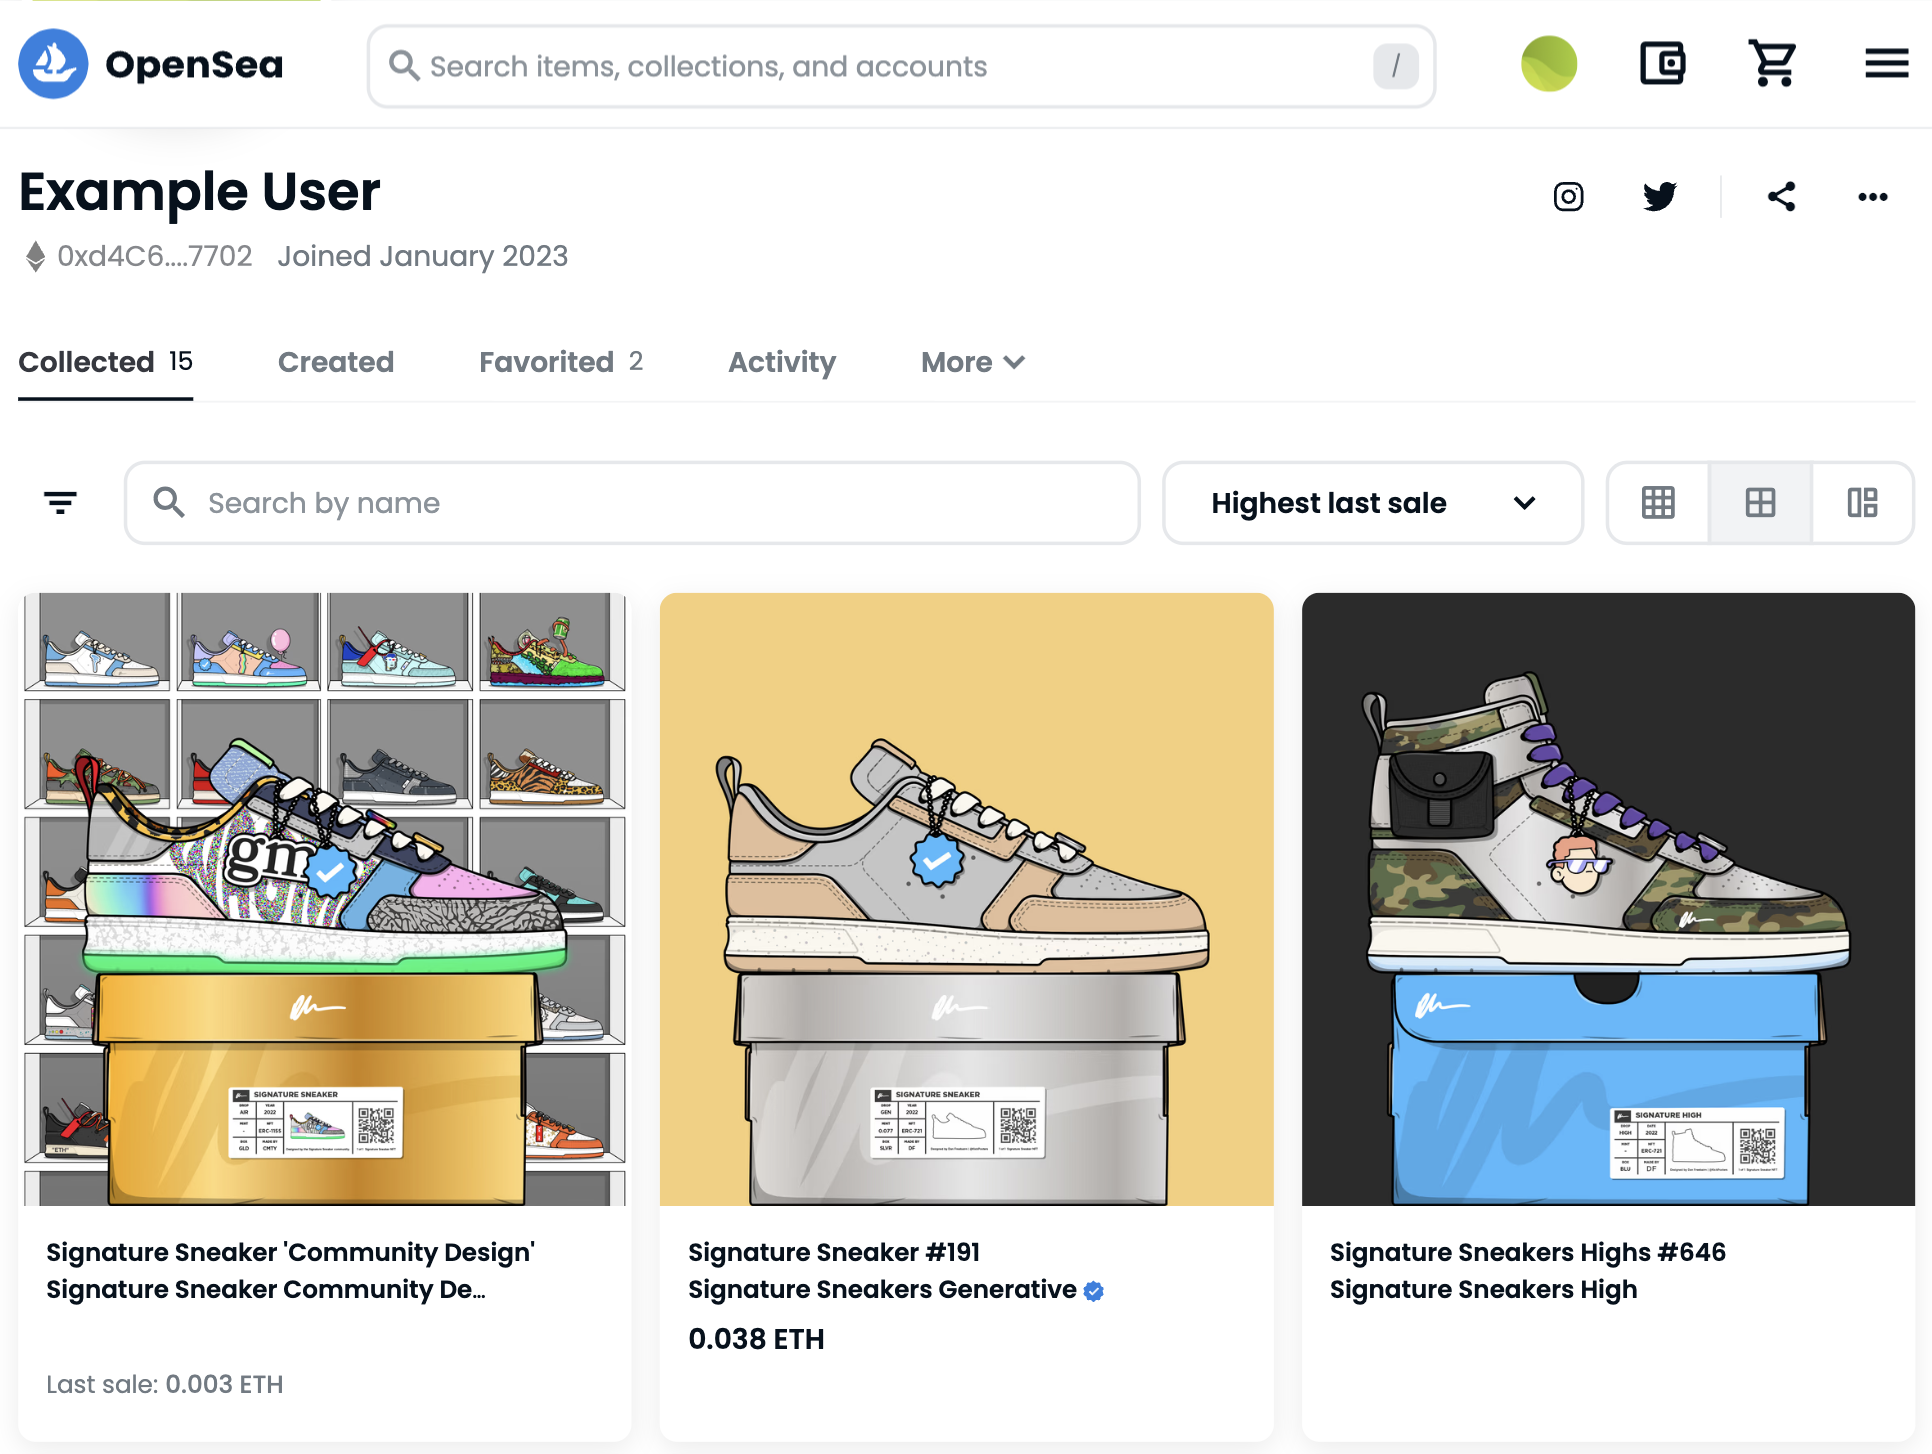
\includegraphics[width=\textwidth]{./gfx/openSea.png}
\centering
\caption{An example profile on the online NFT marketplace \textit{OpenSea} \cite{openSea}.}
\label{fig:openSea}
\end{figure}


You can also see all transactions. Meaning you can see who an individual is interacting with. Using their public address you can gain insight as to what they're buying, selling, etc. which might be useful information of the current user as well.

%
% Section: Obtaining Data Via the Etherscan API
%
\section{Example of Programmatically Obtaining Information Via a Wallet}
\label{sec:methodology:code}
In order to demonstrate that the above information can truly be gathered on any connecting wallet, a short example will be run through. The frontend will be created using React. The example uses the Web3 component library \textit{Rainbow Kit} \cite{rainbowKit}. Using this UI kit, a connect button for wallets is created. The connection to the Ethereum blockchain is created using the React hooks Library named \textit{wagmi}.

When the button is clicked and specified that you wish to connect via MetaMask, the same popup as in figure \ref{fig:metamaskPopup} appears. Once connected, the frontend receives connection details such as the wallet link, the wallet's connection status, and most importantly the public address of the wallet.

Listing \ref{lst:rainbow} shows an example of a simple React component which utilizes the Rainbowkit UI Library. The \textit{ConnectButton} component comes preconfigured with everything necessary to connect a wallet. Therefore, no logic needs to be implemented for a simple connect button.

% Rainbow Kit Connect Wallet
\begin{center}
\begin{lstlisting}[label=lst:rainbow ,language=python, caption=An example of implementing a connect wallet button within the frontend of a webapp using the \textit{RainbowKit} UI Library \cite{rainbowKit}., captionpos=b]

import { ConnectButton } from '@rainbow-me/rainbowkit';

export const YourApp = () => {
  return <ConnectButton />;
};

\end{lstlisting}
\end{center}

Once the wallet has been connected successfully, it is possible to access a variety of information on the wallet. Listing \ref{lst:wagmi} is an example of how \textit{wagmi}, a type of React Hook which utilizes the Ethereum blockchain, is able to retrieve the address of a user. The example then displays the public address in the browser.


% Wagmi Get Public Address
\begin{center}
\begin{lstlisting}[label=lst:wagmi ,language=python, caption=An example of getting a wallet's public address using \textit{wagmi React Hooks for Ethereum} \cite{wagmi}. This can be used once the wallet has been connected successfully., captionpos=b]

import { useAccount } from 'wagmi'
 
function App() {
  const { address, isConnecting, isDisconnected } = useAccount()
 
  if (isConnecting) return <div>Connecting</div>
  if (isDisconnected) return <div>Disconnected</div>
  return <div>{address}</div>
}

\end{lstlisting}
\end{center}

Utilizing the Etherscan API, it is possible to obtain the entire transaction history of any Wallet. Plugging the public address obtained into the API call in listing \ref{lst:apiCall}, it is possible to retrieve user data. The listing contains an example public address used for the purpose of this research.

% Etherscan API get transactions
\begin{center}
\begin{lstlisting}[label=lst:apiCall ,language=python, caption=A real-world example API call made from the frontend in order to retrieve all of a user's transactional data. The API is provided by \textit{Etherscan} \cite{etherscan}., captionpos=b]
https://api.etherscan.io/api?module=account
    &action=tokennfttx
    &contractaddress=0x708E73c7A0D81e00e848c902217d2d39e56d65AF
    &address=${address}
    &page=1&offset=100
    &startblock=0
    &endblock=27025780
    &sort=asc
	&apikey=${apiKey}
\end{lstlisting}
\end{center}

Figure \ref{lst:apiResult} shows the response to the API call in listing \ref{lst:apiCall}. The response is an array of all of the public address's transactions. In this example, only one transaction has been made with the address. The response contains the blockchain's block number, the timestamp when the transaction was written to the blockchain, the public address of the sender (from), the public address of the recipient (to), the name of the token, the token ID, and a variety of information on the gas usage for the transaction.


% Etherscan API transaction result
\begin{center}
\begin{lstlisting}[label=lst:apiResult ,language=python, caption={A real-world example of the response to the API request from listing \ref{lst:apiCall}. The result contains a variety of information, such as the transaction timestamp, the sender's public address (from), and the receivers public address (to). The response is provided by the \textit{Etherscan} API \cite{etherscan}.}, captionpos=b]

[
  {
    "blockNumber": "16526088",
    "timeStamp": "1675159439",
    "hash": "0xdeeb04083dce62a599e4df0050f29eace79a517649dce48b8a1f00961f39742c",
    "nonce": "55820",
    "blockHash": "0x8bcdc1acada5e191ecde74131f3098e42c1d886a48a6edd766425c725d976455",
    "from": "0x36c72892fcc72b52fa3b82ed3bb2a467d9079b9a",
    "contractAddress": "0x708e73c7a0d81e00e848c902217d2d39e56d65af",
    "to": "0xd4c656b454bae586ff3afc28171d2981a1f17702",
    "tokenID": "1009",
    "tokenName": "BoredApeFrens",
    "tokenSymbol": "BAF",
    "tokenDecimal": "0",
    "transactionIndex": "92",
    "gas": "400000",
    "gasPrice": "20873221741",
    "gasUsed": "260812",
    "cumulativeGasUsed": "6383822",
    "input": "deprecated",
    "confirmations": "1357"
  }
]
\end{lstlisting}
\end{center}

Creating this quick example shows that obtaining personal information through a Wallet can easily be achieved. With enough transactions in a user's account, the behavior can be analyzed and used to create content catered toward their interests.

For example, with several transactions in a Wallet's history, it is possible to look at who the user is interacting with. Who are they receiving NFTs from? Who are they sending them to? If they are primarily receiving NFTs from shoe brands, it is feasible to conclude that they have an interests in shoes.

By looking at the token name, the token ID, and the image associated with the token, it is possible to know what the NFT represents. This can be, for example, a specific sneaker from a specific brand.

Even the timestamp of the transaction can be used to gather information. How frequently is the user obtaining NFTs of a shoe? If they are receiving them in consistent time intervals, then that can be used to deliver ads to the user in the timeframe shortly before their next predicted purchase.

With just a few transactions in a Wallet, it is possible to gather behavioral information on a user. The possible applications of this are still in their infant stages. However, the potential can be great. The next chapter will discuss the results of this paper.